\documentclass[11pt,a4paper]{article}
\usepackage[T1]{fontenc}
\usepackage{lmodern}
\usepackage[margin=25mm]{geometry}
\usepackage{microtype,graphicx,booktabs,tabularx,array,amsmath,float,enumitem,xcolor,tikz,listings}
\usetikzlibrary{positioning,arrows.meta,shapes.geometric}
\usepackage{xurl}
\usepackage[hidelinks]{hyperref}
\hypersetup{pdftitle={Air Quality Analytics and Pollution Hotspot Detection in India},pdfsubject={ED547 Big Data Analytics project report}}
\setlength{\parindent}{0pt}
\setlength{\parskip}{7pt}
\setlist[itemize]{leftmargin=18pt,itemsep=3pt,topsep=3pt}
\setlist[enumerate]{leftmargin=20pt,itemsep=3pt,topsep=3pt}
\renewcommand{\arraystretch}{1.2}
\newcolumntype{Y}{>{\raggedright\arraybackslash}X}
\lstset{basicstyle=\ttfamily\small,breaklines=true,frame=single,rulecolor=\color{gray},backgroundcolor=\color{black!3},columns=fullflexible,keepspaces=true}
\newcommand{\units}{\ensuremath{\mu\mathrm{g}/\mathrm{m}^{3}}}
\newcommand{\shot}[3]{\begin{figure}[H]\centering\includegraphics[width=#2\linewidth]{../assets/gray/#1.jpg}\caption{#3}\end{figure}}
\begin{document}
\setcounter{tocdepth}{1}
\tableofcontents
\vspace{15mm}
\textbf{Study scope.} Historical CPCB monitoring observations in India, 1 January to 31 December 2024. This report documents the implemented project and its verified outputs.

\newpage
\section{Introduction and Requirements}
\subsection{Background and problem statement}
Air quality dashboards often emphasize the concentration observed at a particular time. A historical monitoring study also needs to establish whether high pollution repeats and whether enough observations support a comparison. A station with only a few reported days must not appear clean merely because the remaining days are missing.

The project asks: \emph{Which Indian monitoring stations repeatedly experience high pollution during 2024, and how much valid data supports the result?} It uses real measurements from the India Air Quality Database published by XKDR Forum, compiling the CPCB continuous monitoring network [1]. The analysis selects CPCB stations and seven pollutants from twelve monthly bulk files.

\subsection{Objectives}
\begin{itemize}
\item Acquire and reconcile large monthly files with explicit source provenance.
\item Clean observations and calculate pollutant-specific daily comparison metrics.
\item Detect persistent hotspots while showing observation coverage.
\item Compare monthly patterns and individual stations through an interactive dashboard.
\item Execute the analytical SQL in Google BigQuery and verify it independently.
\end{itemize}

\subsection{Application and scope}
The Streamlit application offers pollutant, state/union-territory, city and date filters. It displays monitored locations on a map, ranks stations, shows monthly heatmaps and compares up to three stations. CSV exports allow inspection of the underlying results. A separate combined view summarizes the worst available CPCB severity band.

The project is a historical batch-analysis proof of concept. It does not forecast pollution, ingest live readings, identify emission causes or estimate concentrations at unmonitored places. Monthly differences within one year do not establish recurring multi-year seasonality.

\subsection{Contribution}
The contribution is an auditable combination of persistence screening, explicit missing-data denominators and pollutant-specific rules. Adjustable thresholds and coverage sensitivity make the ranking easier to challenge and explain. This is a focused academic implementation rather than a claim that pollution maps or air quality monitoring are new inventions.

\newpage
\section{Data and Scientific Definitions}
\subsection{Source, selection and record meaning}
The publisher provides monthly Parquet files and station/parameter metadata [1]. The complete acquired 2024 files contain CPCB observations, embassy observations and other chemical parameters. The analytical subset retains CPCB rows for PM2.5, PM10, NO2, SO2, O3, CO and NH3. A record is \emph{one pollutant measurement at one station and time}; counts do not represent that many independent station-hours containing all pollutants.

\begin{table}[H]\centering\caption{Verified data scope}
\begin{tabularx}{\linewidth}{Yr}\toprule
Measure & Executed count\\\midrule
Original monthly files & 12\\
All source measurements acquired & 46,937,170\\
Selected CPCB pollutant measurements & 27,021,875\\
Clean unique pollutant-hour records & 27,021,875\\
Stations in the selected subset & 533\\
Eligible pollutant-station-days & 1,115,522\\
Eligible combined station-days & 165,652\\
Stations without source coordinates & 53\\\bottomrule
\end{tabularx}\end{table}

\subsection{Time, units and missing observations}
Publisher timestamps already represent Indian Standard Time. The ingestion script converts them once to UTC for unique hourly keys, while dates and hours used in the analysis remain IST. This prevents a second timezone conversion from moving observations into the wrong day.

Six pollutants use \units; CO uses $\mathrm{mg}/\mathrm{m}^{3}$. Unit spelling normalization does not alter physical magnitudes. Unexpected units are excluded rather than converted without the required physical information. Raw files remain unchanged, with source filenames and SHA-256 checksums in the acquisition manifest.

No missing readings are filled. Missing, non-finite or negative concentrations are excluded, identical duplicates collapse and conflicting duplicate hours are quarantined. High positive values remain available for inspection. In the executed selected dataset, the hourly cleaning guards removed no rows and found no conflicting duplicate hours. This does not establish that the upstream dataset is error-free.

\subsection{Metadata joins}
Station IDs link measurements to station names, cities, states and coordinates. Left joins preserve stations with incomplete metadata. All 53 stations without coordinates remain eligible for ranking when their observations satisfy the coverage rule. The default PM2.5 selection contains 11 coverage-eligible stations without coordinates, which therefore do not appear on its map.

\newpage
\subsection{Daily eligibility and reference concentrations}
An eligible pollutant-day requires at least 16 valid hourly observations. The comparison metric respects the pollutant's averaging period. For CO and O3, the project takes the highest eligible eight-hour mean within the IST day. Each window needs at least six observations and an endpoint between 07:00 and 23:00 IST. An elapsed-time window prevents gaps from being treated as consecutive hours.

\begin{table}[H]\centering\caption{Individual pollutant screening references}
\begin{tabularx}{\linewidth}{lrlY}\toprule
Pollutant & Reference & Unit & Comparison metric\\\midrule
PM2.5 & 60 & \units & 24-hour mean\\
PM10 & 100 & \units & 24-hour mean\\
NO2 & 80 & \units & 24-hour mean\\
SO2 & 80 & \units & 24-hour mean\\
NH3 & 400 & \units & 24-hour mean\\
O3 & 100 & \units & Highest eligible 8-hour mean\\
CO & 2 & $\mathrm{mg}/\mathrm{m}^{3}$ & Highest eligible 8-hour mean\\\bottomrule
\end{tabularx}\end{table}

A high day exceeds the relevant reference strictly. These short-term references support descriptive screening. They do not implement every legal annual compliance requirement or establish regulatory non-attainment. The government AQI explanation links the relevant ambient standards and documents pollutant averaging periods [2].

\subsection{Combined pollution level}
Each eligible pollutant receives a CPCB concentration band [2]. The displayed ordinal values are 0 Good, 1 Satisfactory, 2 Moderate, 3 Poor, 4 Very Poor and 5 Severe. The combined level for station $s$ and day $d$ is
\[
 L_{s,d}=\max_{p\in P_{s,d}} B_p(c_{s,p,d}),
 \qquad |P_{s,d}|\geq3,
 \qquad P_{s,d}\cap\{\mathrm{PM2.5},\mathrm{PM10}\}\ne\emptyset.
\]
Here $B_p$ maps a comparison concentration to its pollutant band. O3 uses the table's one-hour convention for the upper two bands: a maximum observed hourly value above 208 is Very Poor and above 748 is Severe. Lower bands use the eight-hour comparison value. Classification inputs round to eight decimals to avoid floating-point differences at exact boundaries. Original concentration summaries retain their precision.

This is a derived ordinal screening score, not official numeric AQI, a PCA result or a validated combined health-risk measure. Band differences do not represent equal changes in risk. Lead is unavailable, and missing pollutants can conceal a worse band. The daily details display the available-pollutant count and a defining pollutant, with alphabetical tie-breaking.

\newpage
\section{System Design and Workflow}
\subsection{High-level architecture}
\begin{figure}[H]\centering
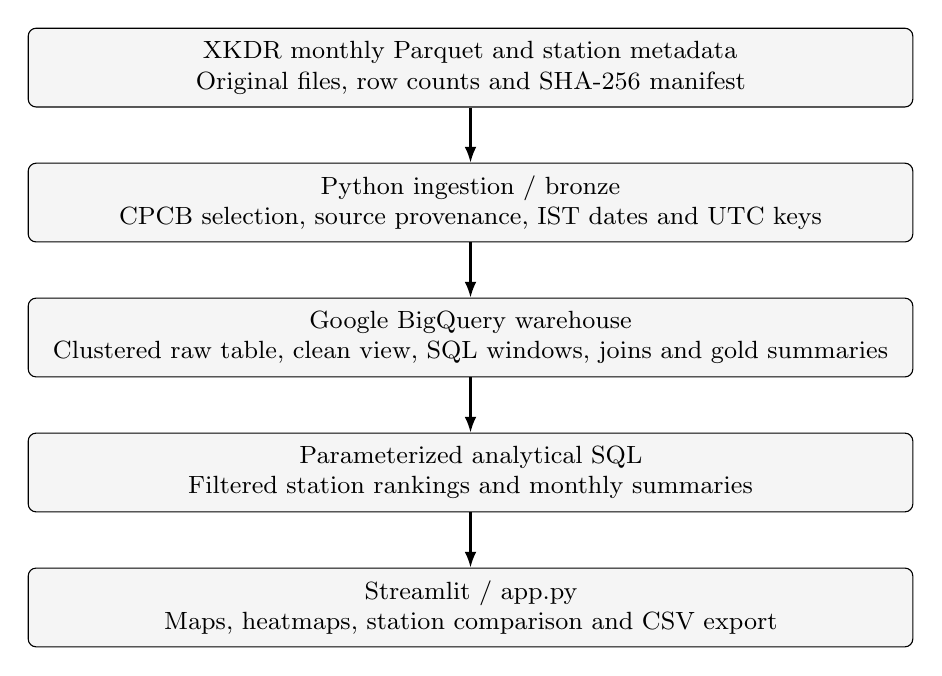
\begin{tikzpicture}[node distance=7mm,box/.style={draw,fill=black!4,rounded corners=1mm,align=center,text width=11cm,minimum height=10mm,font=\small},arr/.style={-{Latex[length=2mm]},thick}]
\node[box] (source) {XKDR monthly Parquet and station metadata\\Original files, row counts and SHA-256 manifest};
\node[box,below=of source] (bronze) {Python ingestion / bronze\\CPCB selection, source provenance, IST dates and UTC keys};
\node[box,below=of bronze] (bq) {Google BigQuery warehouse\\Clustered raw table, clean view, SQL windows, joins and gold summaries};
\node[box,below=of bq] (query) {Parameterized analytical SQL\\Filtered station rankings and monthly summaries};
\node[box,below=of query] (app) {Streamlit / app.py\\Maps, heatmaps, station comparison and CSV export};
\draw[arr] (source)--(bronze);\draw[arr] (bronze)--(bq);\draw[arr] (bq)--(query);\draw[arr] (query)--(app);
\end{tikzpicture}
\caption{Main data path of the academic application. BigQuery performs the dashboard aggregation.}
\end{figure}

\subsection{Independent validation path}
The same bronze inputs also feed DuckDB locally. Local SQL creates partitioned silver Parquet and gold reference outputs. Validation compares the four cloud analytical tables with these independent results, including unique keys, row counts, numerical values and classification flags. DuckDB is a correctness reference, not an alternative application backend.

\subsection{Lifecycle and execution boundaries}
Acquisition preserves the original files. Normalization and cleaning produce reusable analytical layers. Quality checks precede interpretation, and run audits retain execution evidence. The dashboard uses a read-only viewer identity, while owner Application Default Credentials perform warehouse loading and transformations.

The batch workflow uses an ordered Python runner that stops on a failed step. Apache Airflow, streaming systems and prediction models are outside this implemented proof of concept. Their names must not be presented as implemented components.

\newpage
\section{Processing and Algorithm Implementation}
\subsection{SQL processing}
The local and cloud SQL stages check units and concentrations, reconcile duplicate station/pollutant/time keys, create daily metrics and join pollutant references. Grouped summaries calculate monthly and annual results. Station metadata joins preserve analytical row counts.

An eight-hour metric needs a time range rather than the previous eight available rows. Otherwise, missing observations could extend a nominal eight-hour window over a longer period. The cloud hourly stage applies time-based window aggregation; synthetic SQL tests include a long gap to verify this distinction.

\subsection{Coverage and persistence}
For station $s$, let $D$ be the number of calendar days in the selected period, $V_s$ valid observed days and $H_s$ high days. Then
\[
 C_s=100\frac{V_s}{D},\qquad E_s=100\frac{H_s}{V_s}.
\]
Monthly coverage uses the calendar days that overlap the selected period. This preserves the correct denominator for a partial month. Default screening requires overall coverage $C_s\geq75\%$. A month qualifies when it also has at least 75\% coverage and at least 10\% of its observed days are high. A persistent hotspot has at least three qualifying high-pollution months and passes overall coverage.

\begin{lstlisting}
for each station in the selected scope:
    count valid days and high days
    coverage = valid days / calendar days
    for each overlapping calendar month:
        calculate month coverage and high-day fraction
        count month if coverage >= 75% and high fraction >= 10%
    eligible = overall coverage >= 75%
    persistent = eligible and high months >= 3
\end{lstlisting}

The dashboard exposes these thresholds. They are transparent project choices, not official hotspot definitions. In the combined view, a high day means level 3 or above. For an individual pollutant, it means exceeding that pollutant's concentration reference.

\subsection{Application queries}
BigQuery computes filtered rankings and the top-station monthly summaries in SQL. The application downloads at most three selected station series for comparison. Query values use bound parameters, identifiers are validated, each query has a byte ceiling and cached results expire after ten minutes. Failed cloud requests do not silently switch to local results.

\newpage
\section{Dashboard Application}
\subsection{Hotspot map and station ranking}
\shot{dashboard_overview}{1}{Actual dashboard overview for PM2.5, all states, all of 2024 and default thresholds.}
\shot{dashboard_map}{1}{Actual monitored-point map for the same selection, reproduced in grayscale.}

The summary shows 529 stations with PM2.5 results, 416 passing the coverage screen and 342 meeting the persistence rule. The 27.0M measurement indicator describes the complete seven-pollutant study, not the count remaining after every current filter.

The map displays observed monitoring locations rather than a continuous pollution surface. Marker size and shading represent the fraction of valid days above the PM2.5 benchmark. Missing coordinates exclude a station only from the map, not from the ranking. The geographic basemap is a third-party cartographic background, not a project boundary determination.

\newpage
\subsection{Monthly patterns and observation coverage}
\shot{dashboard_monthly}{1}{Actual monthly PM2.5 heatmap for the 15 highest-ranked stations in the default selection.}
\shot{dashboard_coverage}{1}{Actual monthly coverage heatmap for those stations.}

The concentration heatmap displays means of daily comparison values. It masks months below the selected coverage threshold. The second heatmap makes the underlying missingness visible, preventing a blank concentration cell from being mistaken for a clean month.

Several displayed Delhi and Gurugram stations have higher observed concentrations in November and January than in many mid-year months. This is a descriptive finding for the selected stations and year. It cannot establish a recurring seasonal pattern, quantify citywide exposure or identify the cause of the difference. The selection is intentionally the top-ranked subset, not a representative sample of all Indian stations.

\newpage
\subsection{Station comparison and combined view}
\shot{dashboard_comparison}{1}{Actual PM2.5 daily comparison for Gurugram site\_5345 and Byrnihat site\_5669. The dashed line marks 60 \units.}
\shot{dashboard_combined}{1}{Actual combined-view summary with default annual coverage and persistence thresholds.}

Daily comparison aligns stations to the same calendar. Gaps remain gaps, and up to three stations can be selected. The source-derived detail table reports the observations and metrics behind each day, with a CSV export for inspection.

The combined summary contains 532 stations with eligible combined days, 432 coverage-eligible stations and 222 persistent hotspots. Its poor-day criterion differs from the individual pollutant benchmark criterion. These counts therefore must not be interpreted as if they measured the same event. The application explains the minimum-pollutant requirement and the ordinal score beside the view.

\newpage
\section{BigQuery and Course Alignment}
\subsection{Actual warehouse work}
BigQuery stores the selected 27,021,875 hourly measurements and executes cleaning, elapsed-time windows, joins and grouped analytical SQL. The dashboard runs filtered aggregation in the warehouse instead of repeatedly downloading all daily records. The raw table retains source filenames, while the clean hourly layer is a view to avoid another full stored hourly copy.

The executed hourly transformation processed 1,675,996,638 bytes. Its retained job ID is \texttt{510e317a-c81d-46b4-9f0f-b23e8b558e8a}. Cloud job IDs, processed bytes, slot milliseconds and parity records remain in \texttt{data/india/audit/}. These measures establish real cloud execution, not a controlled comparison of elapsed performance.

\subsection{Storage layout and limits}
The Sandbox applies a 60-day expiration rule [3]. Partitioning the uploaded data by its old 2024 event dates would immediately expire historical partitions. The implemented raw table instead uses clustering by pollutant, date and station, with table-level retention. Local silver Parquet remains partitioned by month and pollutant. The cloud project is configured in US as a compute location; its observations remain Indian.

The recorded active logical storage is approximately 2.51 GiB. Tables still expire relative to creation, and a later demonstration may require a rebuild. Query-byte ceilings and a ten-minute dashboard cache limit repeated work. Quotas and retention must be checked before reusing the project.

\begin{table}[H]\centering\caption{Match to ED547 Big Data Analytics}
\begin{tabularx}{\linewidth}{lY}\toprule
Module & Implemented connection\\\midrule
I: Introduction & Volume, variety of pollutant/time/station attributes, veracity, value and lifecycle. Historical batch data gives limited velocity.\\
II: Storage & Cloud analytical warehouse, columnar Parquet, clustered tables and layered data management.\\
III: Frameworks & Batch-processing concepts. Hadoop, Spark, YARN and RDDs are not implemented.\\
IV: Ingestion/ETL & Bulk acquisition, normalization, quality checks and reproducible transformation stages.\\
V: Analytics tools & Google BigQuery, SQL and Python scripting. Ordered scripts provide simple orchestration; Airflow is not implemented.\\\bottomrule
\end{tabularx}\end{table}

BigQuery is useful for warehouse execution and a lightweight hosted dashboard. A capable laptop can also process this dataset, as the DuckDB reference demonstrates. The project does not claim that the data is beyond every laptop's capacity or that BigQuery is necessarily faster.

\newpage
\section{Analytical Results}
\subsection{Default annual screening}
Table~\ref{tab:results} reports observed station counts for the complete 2024 study period. Eligibility requires at least 75\% valid-day coverage. Persistence requires at least three adequately observed months with 10\% or more high days.

\begin{table}[H]\centering\caption{Coverage-eligible stations and persistent hotspots}\label{tab:results}
\begin{tabular}{lrr}\toprule
Analysis view & Coverage eligible & Persistent\\\midrule
PM2.5 & 416 & 342\\
PM10 & 412 & 372\\
NO2 & 425 & 35\\
SO2 & 432 & 4\\
O3 & 421 & 167\\
CO & 435 & 172\\
NH3 & 389 & 0\\
Combined level & 432 & 222\\\bottomrule
\end{tabular}\end{table}

Among eligible stations, Sector-51, Gurugram (site\_5345) has the highest PM2.5 exceedance fraction: 84.2\%, based on 330 valid days. Wazirpur, Delhi has the highest PM10 fraction: 96.9\%, based on 358 valid days. These comparisons concern the monitored station, selected pollutant, period and rule. They do not establish that either whole city is the worst in India.

The NH3 result of zero persistent hotspots means that none meets the chosen persistence definition. It does not imply that ammonia is absent or harmless. Different pollutants have different observation availability, reference values and eligible station sets. Their persistent counts are not interchangeable measures of health burden.

\subsection{Coverage sensitivity}
\begin{table}[H]\centering\caption{PM2.5 sensitivity to the minimum coverage threshold}
\begin{tabular}{rrr}\toprule
Minimum coverage & Eligible stations & Persistent hotspots\\\midrule
60\% & 459 & 370\\
75\% & 416 & 342\\
90\% & 297 & 250\\\bottomrule
\end{tabular}\end{table}

Stricter coverage removes stations from the eligible set and changes the persistence count. This makes the observation-support tradeoff visible. It does not demonstrate improving air quality. The dashboard recalculates monthly eligibility with the same selected coverage threshold.

\newpage
\section{Testing and Discussion}
\subsection{Automated validation}
The final cleanup run passed 32 tests. They cover analytical rules, SQL edge cases, validated query construction and live Streamlit workflows. The suite exercises all seven individual pollutants, the combined view, Delhi filtering and a short date interval. Upstream BigQuery DataFrame deprecation warnings remain; the tested functions completed successfully.

\begin{itemize}
\item Duplicate collapse, conflicting-value quarantine and negative concentration exclusion.
\item Minimum daily observations and time-range windows across missing hours.
\item Concentration boundaries, combined pollutant requirements and valid level bounds.
\item Calendar-day denominators, partial periods and persistence thresholds.
\item Bound SQL values, rejected identifiers/filter shapes and historical Sandbox layout.
\end{itemize}

\subsection{Independent cloud-result checks}
The cloud pipeline validated station\_daily, overall\_daily, station\_monthly and station\_annual against the local reference. Numerical comparisons use a tolerance of $10^{-8}$, while classifications and flags match exactly. Three additional dashboard-query scenarios matched the local aggregation:

\begin{table}[H]\centering\caption{Dashboard aggregation parity scenarios}
\begin{tabularx}{\linewidth}{Yrr}\toprule
Selection & Stations & Monthly rows\\\midrule
National PM2.5, full year & 529 & 180\\
National combined level, full year & 532 & 180\\
Delhi O3, 12 February to 19 May & 39 & 60\\\bottomrule
\end{tabularx}\end{table}

The national monthly result contains at most 15 station rows per month, giving 180 rows over twelve months. Station comparison requests retrieve only the selected series. This is a concrete reduction in application-side transfer, not evidence of a universal speed advantage. The two engines share the methodological specification, so parity does not independently validate that specification or sensor accuracy.

\subsection{Reproduction and individual preparation}
\begin{lstlisting}
python -m pip install -r requirements.txt
python -m streamlit run app.py
python -m pytest tests -q
\end{lstlisting}
Private viewer credentials and existing cloud tables are required. The setup guide documents rebuilding the source/reference/cloud pipeline. Work can be demonstrated individually as acquisition/provenance, warehouse SQL, analysis/validation and dashboard/integration. Every member should understand the shared denominators, combined-score definition and limitations.

\newpage
\section{Conclusion and References}
\subsection{Conclusion}
The project turns large-scale Indian monitoring observations into reproducible, coverage-aware historical screening results. Its pipeline acquires and reconciles twelve monthly files, retains 27 million CPCB pollutant measurements, executes the transformations in BigQuery and validates the analytical outputs locally. The dashboard connects national filtering with station-level evidence, monthly coverage and CSV exports.

The main analytical result is that the selected persistence rule identifies 342 PM2.5 hotspots among 416 coverage-eligible stations, while the combined Poor-or-worse screen identifies 222 among 432 eligible stations. These figures describe different criteria. Explicit coverage denominators and sensitivity checks help prevent missing observations from creating misleading clean-day conclusions.

\subsection{Limitations and future work}
\begin{itemize}
\item One historical year supports within-year patterns, not forecasts or recurring multi-year seasonal conclusions.
\item Station locations and reporting schedules do not represent all people or all places. Missing days and pollutants can bias comparisons.
\item Fifty-three stations lack coordinates. Their ranking results remain available, but their map locations cannot be shown.
\item The combined level is a derived ordinal screen, with unavailable lead measurements. It is not official numeric AQI or an exposure/health model.
\item Screening thresholds are project choices. Negative-value exclusion and upstream quality decisions can affect the results.
\item Sandbox retention, quotas, authentication and internet access constrain later demonstrations. No production availability guarantee applies.
\end{itemize}

Useful extensions are another full year for repeat-pattern checks, refreshed station metadata and explicit uncertainty summaries. Weather or emissions data would be needed before investigating pollution causes. These extensions should preserve the project's transparent and limited academic scope.

\subsection*{References}
\addcontentsline{toc}{subsection}{References}
\begin{enumerate}[label={[\arabic*]}]
\item XKDR Forum. \emph{India Air Quality Database}. CPCB CAAQM compilation, CC BY 4.0. \url{https://airquality.xkdr.org/}.
\item Indian Economic Service, Government of India. \emph{National Air Quality Index}. Breakpoints, averaging periods and linked ambient standards. \url{https://ies.gov.in/arthapedia/concept/national-air-quality-index}.
\item Google Cloud. \emph{Try BigQuery using the sandbox}. \url{https://docs.cloud.google.com/bigquery/docs/sandbox}.
\end{enumerate}
\small All web references accessed 1 November 2026. Project results derive from the retained run audits and exported analytical tables.
\end{document}
